\subsection{Online Implementation and End-to-End Evaluation} \label{sec:online}

We implemented \name{}, an FDE generation and end-to-end retrieval engine in C++. 
%in a proprietary codebase. 
%
%To enable reproducibility, we will publish a standalone open-source shared-memory implementation of the FDE generation step upon publication.
We discussed FDE generation and various optimizations and their tradeoffs in (§\ref{sec:fde-experimental}). %
Next, we discuss how we perform retrieval over the FDEs, and additional optimizations.

\paragraph{Single-Vector MIPS Retrieval using DiskANN}
Our single-vector retrieval engine uses a scalable implementation~\cite{parlayann} of DiskANN~\cite{diskann} (MIT License), a state-of-the-art graph-based ANNS algorithm.
%We use DiskANN as it (along with other graph-based algorithms) empirically has a much better tradeoff between recall and QPS (and latency) compared with other ANNS techniques, e.g., hashing (LSH) or clustering-based approaches.
We build DiskANN indices by using the uncompressed document FDEs with a maximum degree of 200 and a build beam-width of 600.
Our retrieval works by querying the DiskANN index using beam search with beam-width $W$, and subsequently reranking the retrieved candidates with Chamfer similarity.
The only tuning knob in our system is $W$; increasing $W$ increases the number of candidates retrieved by \name{}, which improves the recall.

\paragraph{Ball Carving.} To improve re-ranking speed, we reduce the number of query embeddings by clustering them via a {\em ball carving} method and replacing the embeddings in each cluster with their sum. 
This speeds up reranking without decreasing recall; we provide further details in (§\ref{apx:ballcarve}).


\paragraph{Product Quantization (PQ).}
To further improve the memory usage of $\name$, we use a textbook vector compression technique called product quantization (PQ) with asymmetric querying~\cite{jegou2010product, guo2020accelerating} on the FDEs. %with asymmetric querying~\cite{jegou2010product, guo2020accelerating}; 
We refer to product quantization with $C$ centers per group of $G$ dimensions as $\mathsf{PQ}\text{-}C\text{-}G$. For example, $\mathsf{PQ}\text{-}256\text{-}8$, which we find to provide the best tradeoff between quality and compression in our experiments, compresses every consecutive set of $8$ dimensions to one of $256$ centers. Thus $\mathsf{PQ}\text{-}256\text{-}8$  provides $32\times$ compression over storing each dimension using a single float, since each block of $8$ floats is represented by a single byte. See (§\ref{apx:PQ}) for further experiments and details on PQ.


\paragraph{Experimental Setup}
We run our online experiments on an Intel Sapphire Rapids machine on Google Cloud (c3-standard-176). The machine supports up to 176 hyper-threads. 
We run latency experiments using a single thread, and run our QPS experiments on all 176 threads.


\begin{figure*}[t]
\vspace{-2em}
  \subfloat{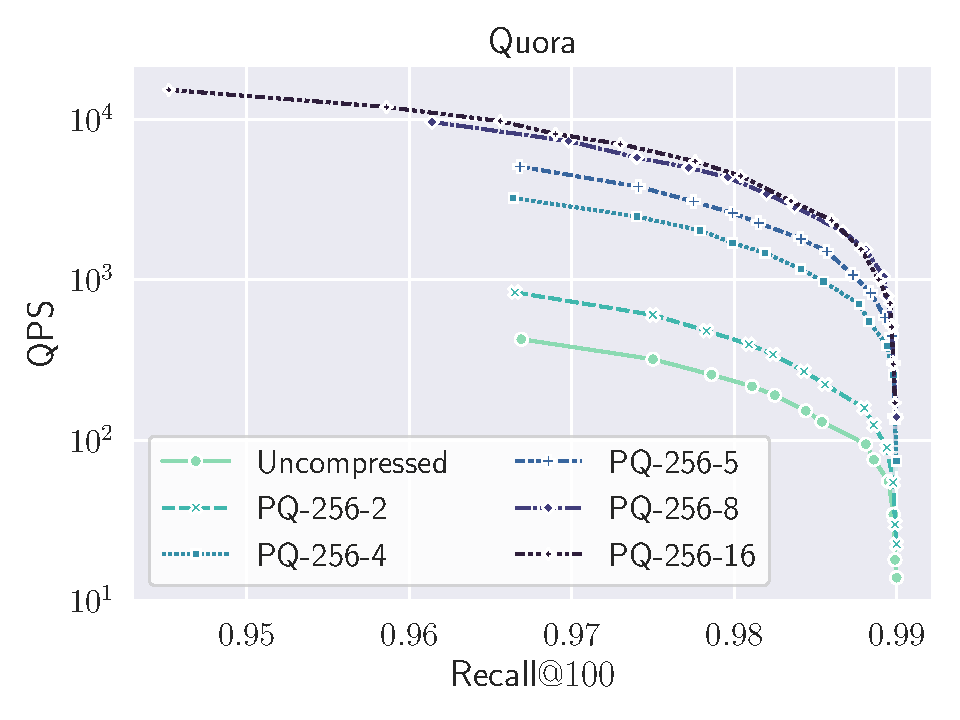
\includegraphics[width=.33\linewidth]{plots/pq_vs_qps_100/quora-pq_vs_nopq.pdf}} 
  \subfloat{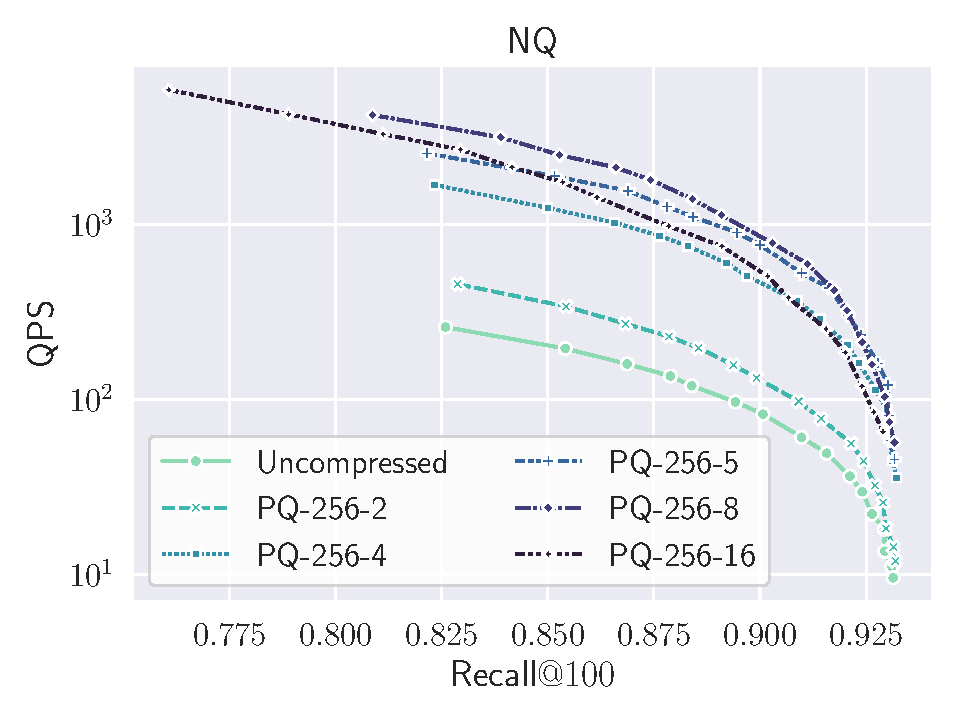
\includegraphics[width=.33\linewidth]{plots/pq_vs_qps_100/nq-pq_vs_nopq.pdf}} 
  \subfloat{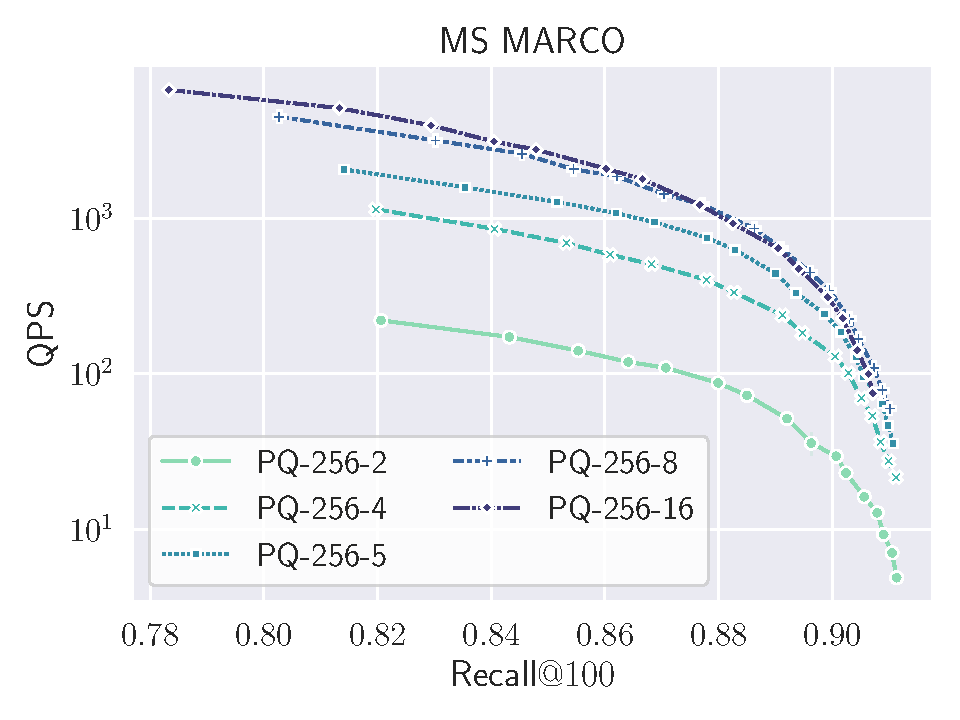
\includegraphics[width=.33\linewidth]{plots/pq_vs_qps_100/msmarco-pq_vs_nopq.pdf}}
  
\vspace{-1em}
  \caption{\small Plots showing the QPS vs. Recall@$100$ for \name{} on a subset of the BEIR datasets. The different curves are obtained by using different PQ methods on 10240-dimensional FDEs.}
\label{fig:qpsvsrecall100}
\end{figure*}
\paragraph{QPS vs. Recall}
A useful metric for retrieval is the number of {\em queries per second (QPS)} a system can serve at a given recall; evaluating the QPS of a system tries to fully utilize the system resources (e.g., the bandwidth of multiple memory channels and caches), and deployments where machines serve many queries simultaneously. 
Figure~\ref{fig:qpsvsrecall100} shows the QPS vs. Recall@100 for \name{} on a subset of the BEIR datasets, using different PQ schemes over the FDEs. We show results for additional datasets, as well as Recall@1000, in the Appendix.
Using $\mathsf{PQ}\text{-}256\text{-}8$ not only reduces the space usage of the FDEs by 32$\times$, but also improves the QPS at the same query beamwidth by up to 20$\times$, while incurring a minimal loss in end-to-end recall.
Our method has a relatively small dependence on the dataset size, which is consistent with prior studies on graph-based ANNS data structures, since the number of distance comparisons made during beam search grows roughly logarithmically with increasing dataset size~\cite{parlayann, diskann}. 
We tried to include QPS numbers for PLAID~\cite{santhanam2022plaid}, but unfortunately their implementation does not support running multiple queries in parallel, and is optimized for measuring latency.



\begin{figure*}[t]
%\vspace{-1em}
%\subfigure[Figure A]{\label{fig:a}\includegraphics[width=60mm]{example-image-a}}
  \centering
 % \vspace{-1.5em}
  \subfloat{
    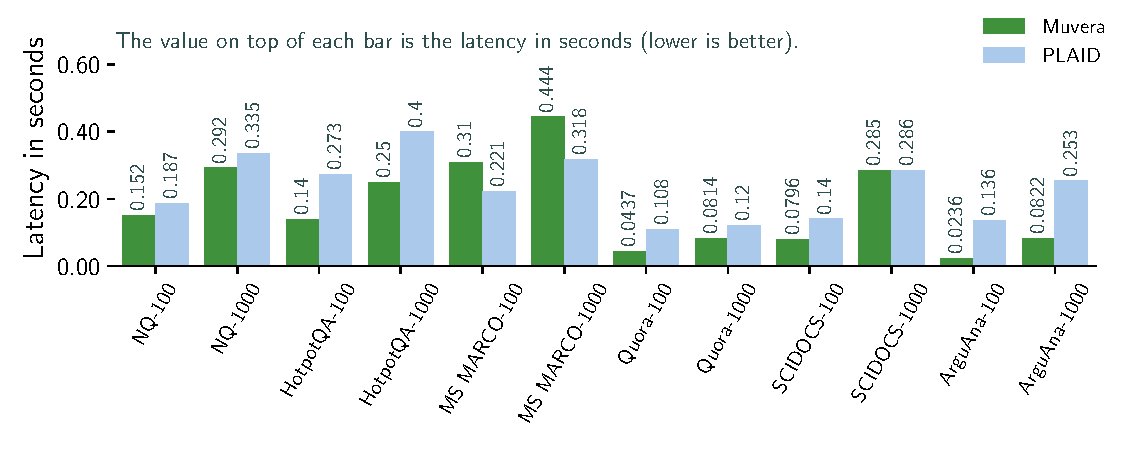
\includegraphics[width=.8\linewidth]{plots/latency-bar.pdf}} \\
 %  \vspace{-1.5em} 
  \subfloat{
    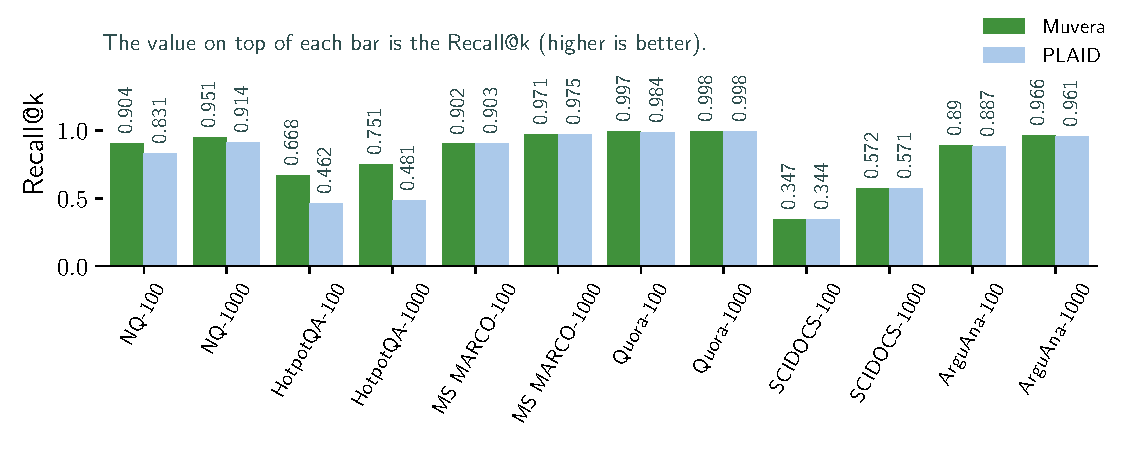
\includegraphics[width=.8\linewidth]{plots/recall-bar.pdf}}
%\vspace{-1em}
  \caption{\small Bar plots showing the latency and Recall@$k$ of \name{} vs PLAID on a subset of the BEIR datasets. The x-tick labels are formatted as dataset-$k$, i.e., optimizing for Recall@$k$ on the given dataset. \label{fig:vsplaid}}
\end{figure*}
\paragraph{Latency and Recall Results vs. PLAID~\cite{santhanam2022plaid}}
We evaluated \name{} and PLAID~\cite{santhanam2022plaid} on the 6 datasets from the BEIR benchmark described earlier in (§\ref{sec:eval}); Figure~\ref{fig:vsplaid} shows that \name{} achieves essentially equivalent Recall@$k$ as PLAID (within 0.4\%) on MS MARCO, while obtaining up to 1.56$\times$ higher recall on other datasets (e.g. HotpotQA).
We ran PLAID using the recommended settings for their system, which reproduced their recall results for MS MARCO.
Compared with PLAID, on average over all $6$ datasets and $k \in \{100,1000\}$, \name{} achieves 10\% higher  Recall@$k$ (up to 56\% higher), and 90\% lower latency (up to 5.7$\times$ lower).



Importantly, \name{} has consistently high recall and low latency across all of the datasets that we measure, and our method {\em does not} require costly parameter tuning to achieve this---all of our results use the same 10240-dimensional FDEs that are compressed using PQ with $\mathsf{PQ}\text{-}256\text{-}8$; the only tuning in our system was to pick the first query beam-width over the $k$ that we rerank to that obtained recall matching that of PLAID. As Figure~\ref{fig:vsplaid} shows, in cases like NQ and HotpotQA, \name{} obtains much higher recall while obtaining lower latency. Given these results, we believe a distinguishing feature of \name{} compared to prior multi-vector retrieval systems is that it achieves consistently high recall and low latency across a wide variety of datasets with minimal tuning effort.

